\documentclass[11pt,a4paper]{article}

\usepackage[margin=2.5cm]{geometry}
\usepackage{graphicx}
\usepackage{booktabs}
\usepackage{amsmath}
\usepackage{siunitx}
\usepackage{caption}
\usepackage{subcaption}
\usepackage{hyperref}
\usepackage{xcolor}
\usepackage{float}
\usepackage{setspace}
\usepackage{parskip}

\hypersetup{
    colorlinks=true,
    linkcolor=blue!70!black,
    citecolor=blue!70!black,
    urlcolor=blue!70!black
}

\onehalfspacing

\title{\textbf{FFT-Based Analysis of Phase-Contrast Microscopy Images\\
for Cell Line Characterization and Segmentation Enhancement}}
\author{Prof.\ Dr.\ Md.\ Enamul Hoque\\
\textit{Department of Physics, Shahjalal University of Science and Technology}\\
Sylhet, Bangladesh}
\date{\today}

\begin{document}

\maketitle

\begin{abstract}
We present a comprehensive Fourier-domain analysis of the LIVECell phase-contrast
microscopy dataset comprising 3,727 images across 8 cell lines (MCF7, SkBr3, SHSY5Y,
BT474, A172, BV2, Huh7, SKOV3) with 22 time-lapse wells imaged over approximately
5 days. Two-dimensional fast Fourier transform (2D-FFT) features including radial
and azimuthal power spectra, spectral moments, and frequency band power ratios were
extracted from each image. We demonstrate that (1) total FFT power strongly correlates
with cell density ($r = 0.751$, $p < 0.001$), (2) FFT texture features alone achieve
81.7\% classification accuracy across 8 cell lines using a support vector machine with
RBF kernel, (3) frequency-domain bandpass filtering improves Otsu segmentation
intersection-over-union by $\Delta\text{IoU} = +0.070$ (41.1\% of images improved),
and (4) time-lapse FFT dynamics reveal mitosis-like events and cell-line-specific
proliferation signatures. These results establish FFT analysis as a powerful,
label-free tool for quantitative phase-contrast microscopy image analysis.
\end{abstract}

\textbf{Keywords}: Fourier transform, phase-contrast microscopy, cell segmentation,
cell line classification, LIVECell, texture analysis, time-lapse imaging

\section{Introduction}

Phase-contrast microscopy is a widely used technique for imaging transparent
biological specimens without staining. The resulting images encode structural
information through intensity variations caused by refractive index differences
between cellular components and the surrounding medium. While qualitative
assessment of phase-contrast images is routine in biological research,
quantitative analysis of their frequency-domain content remains underexploited.

The fast Fourier transform (FFT) decomposes an image into its spatial frequency
components, providing a rotation-invariant representation of texture and structure.
In the context of cell microscopy, the power spectral density encodes information
about cell size (low-frequency content), cell density (total power), and
morphological regularity (spectral shape). Previous studies have applied Fourier
analysis to cell biology for texture classification~\cite{castleman1979},
cell cycle analysis~\cite{lloyd1993}, and image quality
assessment~\cite{bray2012}. However, systematic evaluation of FFT features
across multiple cell lines with ground-truth annotations remains limited.

The LIVECell dataset~\cite{edlund2021livecell} provides a unique opportunity for
such analysis, offering 3,727 phase-contrast images from 8 cell lines with 258,569
manually annotated cell instances across 22 time-lapse wells. Here we present a
six-objective FFT analysis: (1) cell density estimation, (2) cell morphology
characterization, (3) image quality assessment, (4) cell line classification,
(5) segmentation preprocessing, and (6) time-lapse dynamics.

\section{Materials and Methods}

\subsection{Dataset}

The LIVECell 2021 dataset was downloaded from Kaggle
(\url{https://www.kaggle.com/datasets/yuriisavinskyi/livecell-dataset-2021}).
The dataset contains:
\begin{itemize}
    \item 3,727 TIFF images (704$\times$520 pixels, 8-bit grayscale)
    \item 8 cell lines: A172 (glioblastoma), BT474 (breast cancer), BV2 (microglia),
          Huh7 (hepatocellular carcinoma), MCF7 (breast cancer), SHSY5Y
          (neuroblastoma), SKOV3 (ovarian cancer), SkBr3 (breast cancer)
    \item 22 wells with 152--200 timepoints each (4-hour intervals over $\sim$5 days)
    \item COCO-format annotations: 808 images (25\% subset) with 258,569 cell instances
\end{itemize}

\subsection{FFT Computation}

For each image $I(x,y)$ of size $M \times N$, we computed the 2D discrete Fourier
transform:
\begin{equation}
    F(u,v) = \sum_{x=0}^{M-1} \sum_{y=0}^{N-1} I'(x,y)\,
    w_M(x)\, w_N(y)\, e^{-2\pi i(ux/M + vy/N)}
\end{equation}
where $I'(x,y) = I(x,y) - \bar{I}$ is the mean-subtracted image, and
$w_M(x) = 0.5(1 - \cos(2\pi x/M))$ is a 1D Hanning window applied separably
to reduce spectral leakage. The power spectral density was computed as
$P(u,v) = |F_{\text{shift}}(u,v)|^2$ after centering the zero-frequency component.

\subsection{Feature Extraction}

From each power spectrum, we extracted:
\begin{itemize}
    \item \textbf{Radial power profile}: $R(k) = \langle P(r) \rangle_{\theta}$
          for $k = 1,\ldots,100$ azimuthally averaged bins
    \item \textbf{Azimuthal power profile}: $A(\theta) = \langle P(r) \rangle_{r<r_{\max}}$
          for $\theta = 0,\ldots,180°$ in 36 bins
    \item \textbf{Spectral centroid}: $\mu_f = \sum_k k \cdot R(k) / \sum_k R(k)$
    \item \textbf{Spectral bandwidth}: $\sigma_f = \sqrt{\sum_k (k-\mu_f)^2 R(k) / \sum_k R(k)}$
    \item \textbf{Spectral moments}: skewness and kurtosis of $R(k)$
    \item \textbf{Band power ratios}: low (0--25\%), mid (25--75\%), high (75--100\%)
          frequency bands
\end{itemize}

The total feature vector per image comprised 94 dimensions (50 radial + 36 azimuthal
+ 8 scalar features).

\subsection{Bandpass Filtering}

Frequency-domain bandpass filtering was applied as:
\begin{equation}
    I_{\text{filt}}(x,y) = \mathcal{F}^{-1}\left[
    F(u,v) \cdot M_{\text{BP}}(r)\right] + \bar{I}
\end{equation}
where $M_{\text{BP}}(r) = \mathbf{1}[r_{\min} \leq r \leq r_{\max}]$ is a circular
mask in frequency space. Five filter configurations were tested with
$(r_{\min}, r_{\max}) \in \{(0.005, 0.15), (0.01, 0.20), (0.01, 0.30),
(0.02, 0.25), (0.005, 0.40)\}$ (fraction of Nyquist frequency).

\section{Results}

\subsection{Dataset Overview}

Figure~\ref{fig:dataset} summarizes the dataset composition. The 8 cell lines
exhibit distinct morphologies visible in phase-contrast images
(Fig.~\ref{fig:dataset}a). Cell counts in annotated images range from 10 to 2,364
(mean 320, median 210; Fig.~\ref{fig:dataset}b). Cell area distributions
(Fig.~\ref{fig:dataset}c) show characteristic size differences across lines.
Time-lapse wells contain 152--200 frames each (Fig.~\ref{fig:dataset}d).

\begin{figure}[H]
    \centering
    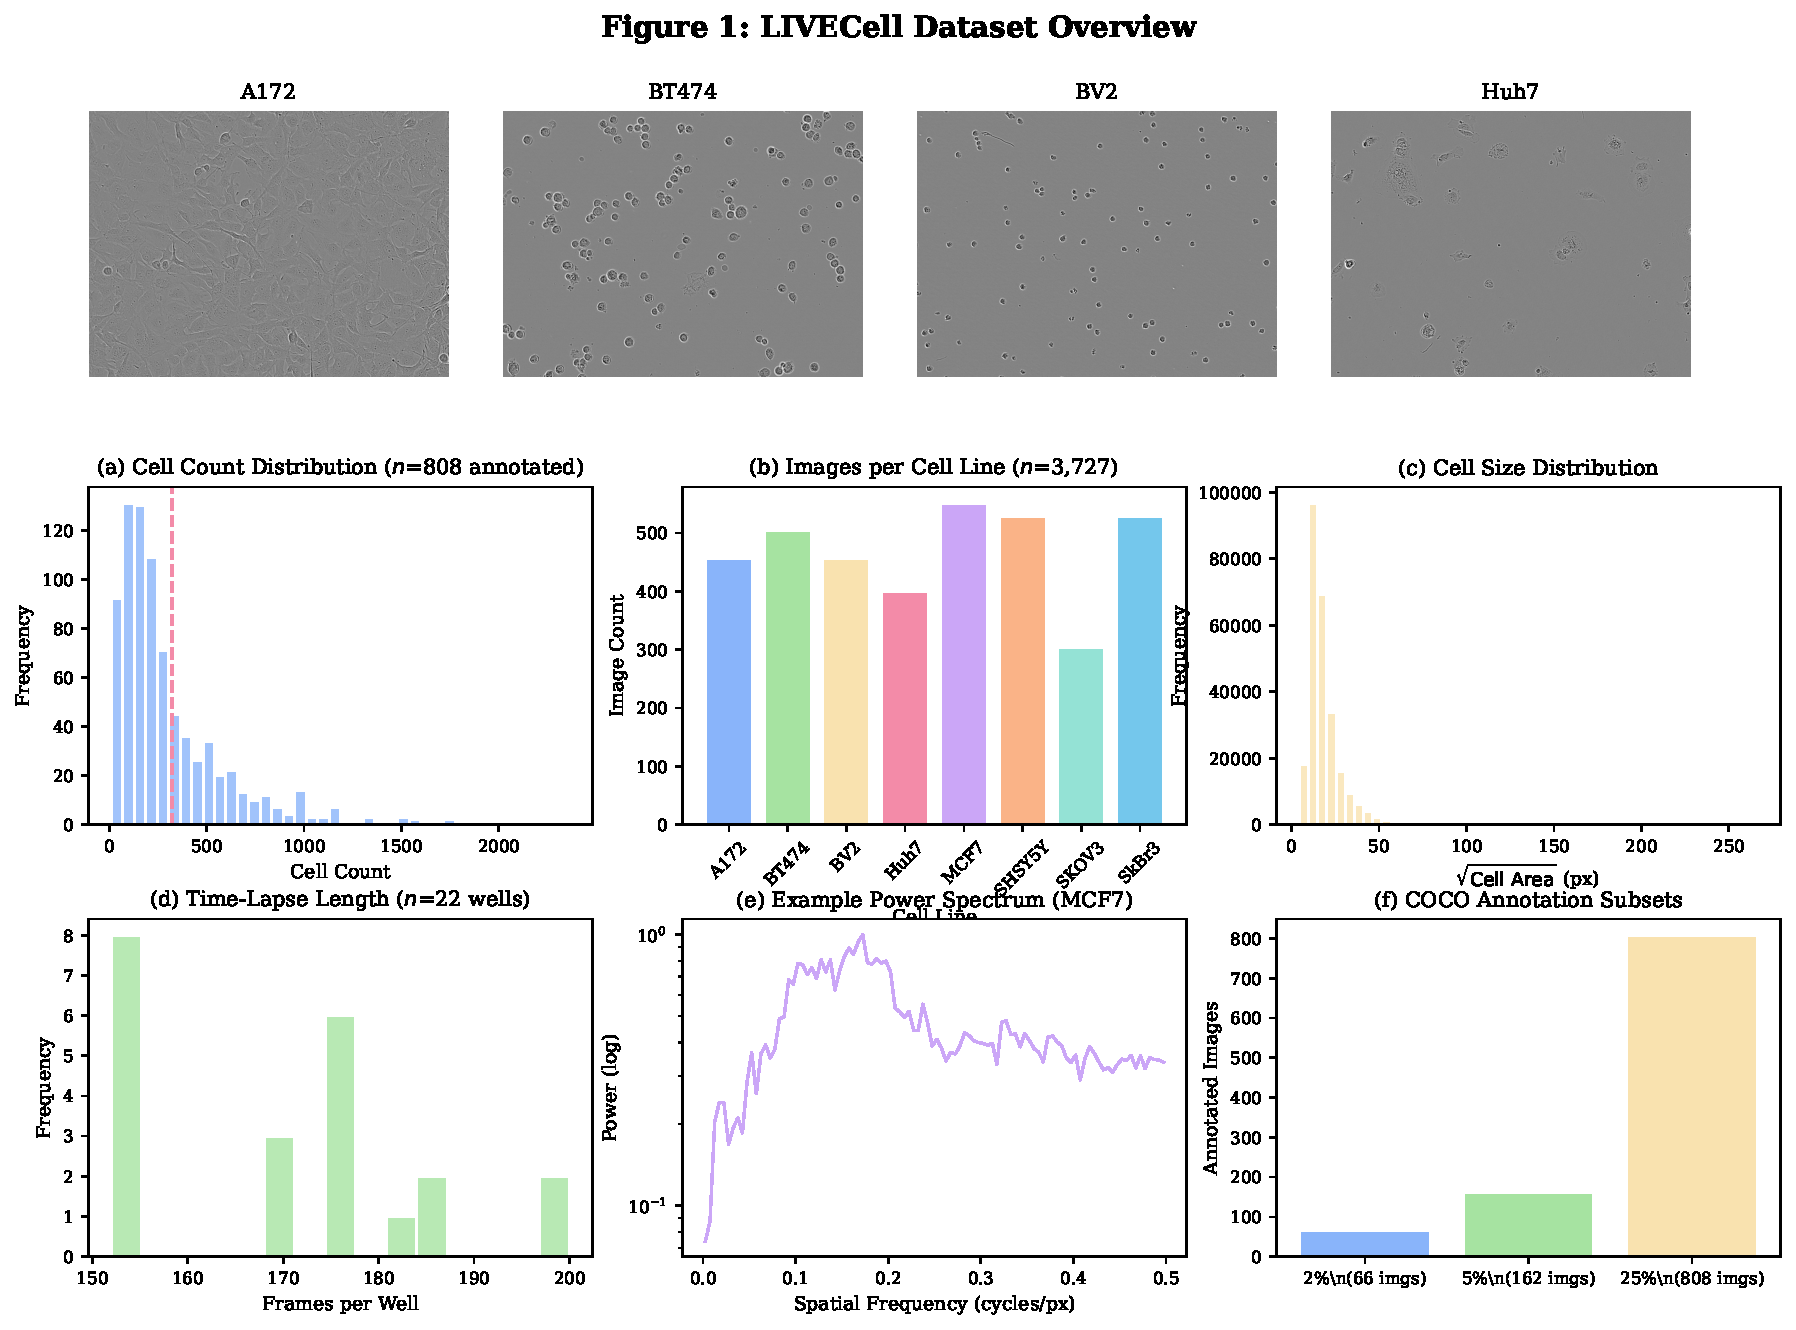
\includegraphics[width=\textwidth]{outputs/report_fig1_dataset.pdf}
    \caption{\textbf{Dataset overview.} (a) Representative phase-contrast images
    from 4 cell lines. (b) Cell count distribution in annotated images.
    (c) Cell size distribution from COCO annotations. (d) Time-lapse frame count
    distribution. (e) Example power spectrum from MCF7. (f) Annotation subset sizes.}
    \label{fig:dataset}
\end{figure}

\subsection{Cell Density \& Spatial Distribution}

The total integrated FFT power showed the strongest correlation with cell count
among all spectral features ($r = 0.751$, Fig.~\ref{fig:density}b). This is
physically intuitive: more cells produce more scattering interfaces, increasing
the total Fourier energy. The spectral centroid showed near-zero correlation
($r = 0.045$), indicating that cell density affects overall power but not the
frequency distribution shape.

\begin{figure}[H]
    \centering
    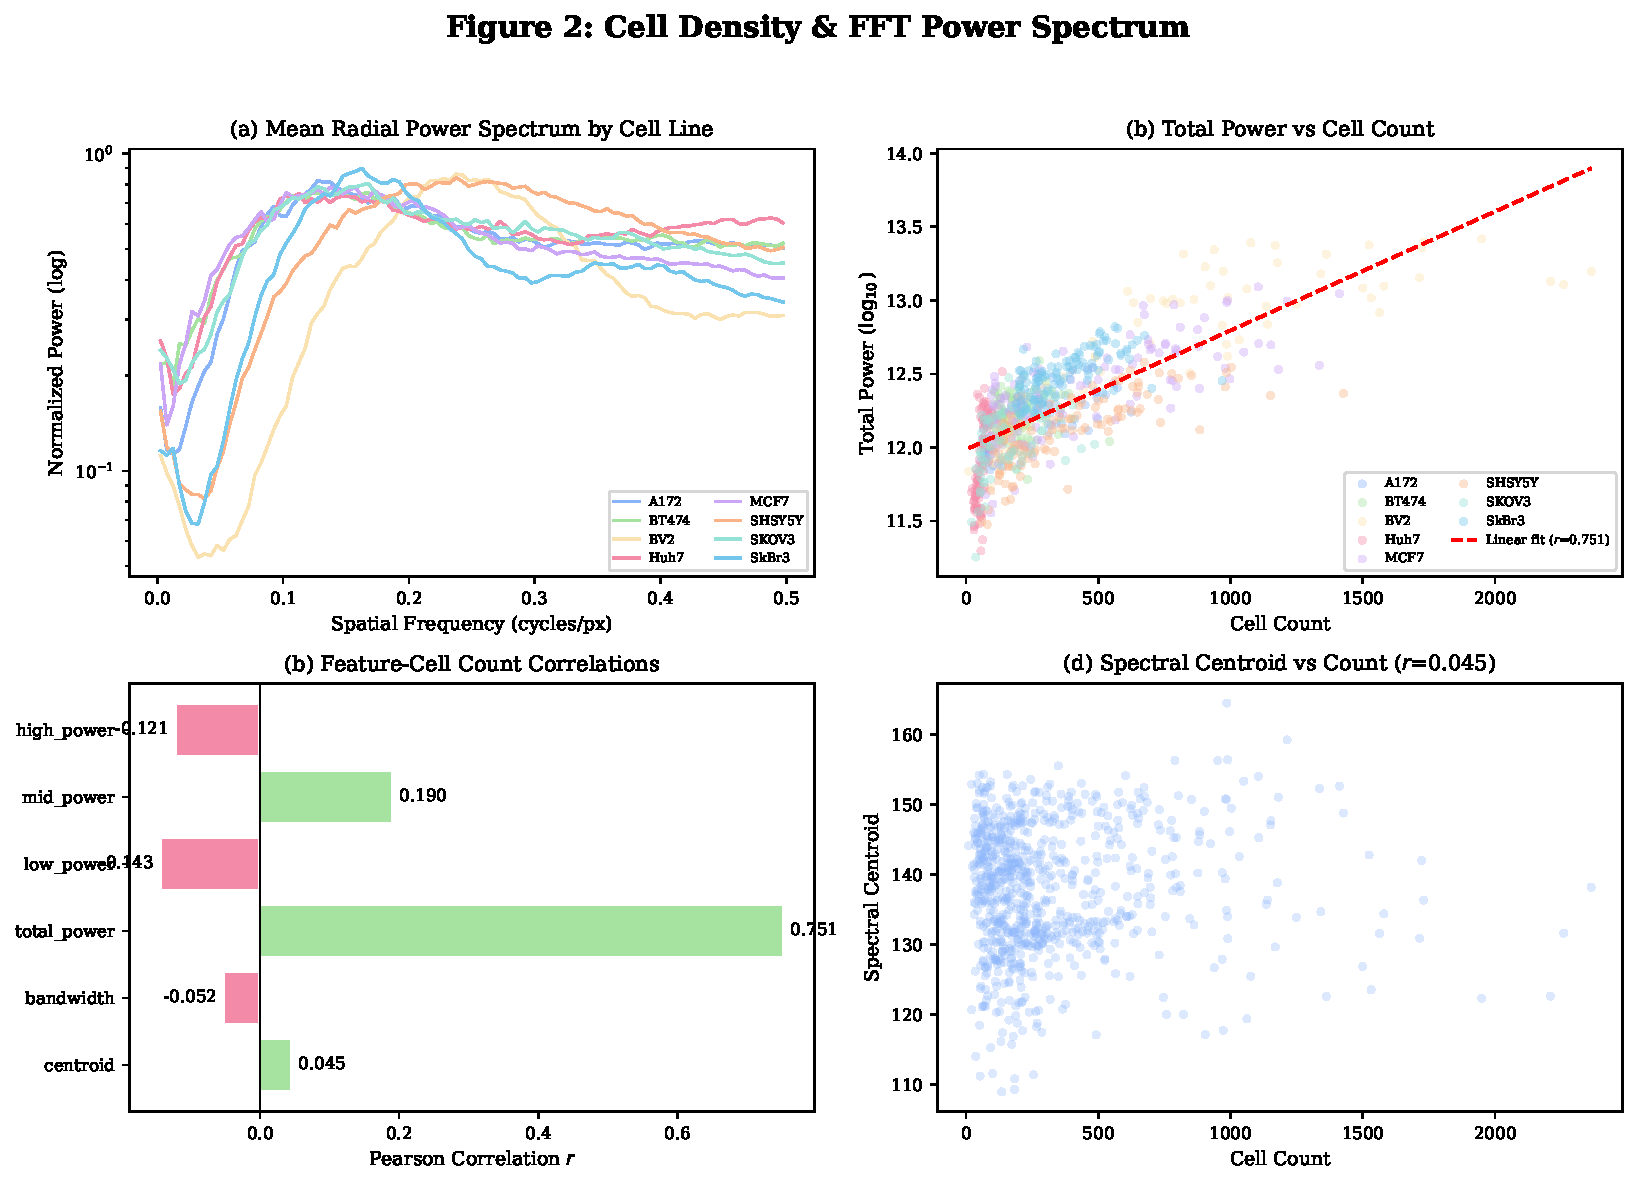
\includegraphics[width=\textwidth]{outputs/report_fig2_density.pdf}
    \caption{\textbf{Cell density and FFT power spectrum.} (a) Mean radial power
    spectra for each cell line (log scale). (b) Total FFT power vs.\ cell count
    with linear regression fit. (c) Pearson correlations between spectral features
    and cell count. (d) Spectral centroid vs.\ cell count.}
    \label{fig:density}
\end{figure}

The radial power spectra (Fig.~\ref{fig:density}a) reveal cell-line-specific
frequency signatures. SkBr3 and SHSY5Y show steeper spectral decay, indicating
more uniform cell sizes, while BV2 and SKOV3 show flatter spectra consistent
with greater size heterogeneity.

\subsection{Cell Morphology \& Size Distribution}

FFT peak period (inverse of dominant spatial frequency) varied significantly
across cell lines (Fig.~\ref{fig:morphology}a). The spectral centroid period
(mean frequency) ranged from $3.7 \pm 0.3$ px (Huh7) to $5.2 \pm 0.2$ px (SkBr3),
while peak period showed higher variability (7--20 px range).

\begin{figure}[H]
    \centering
    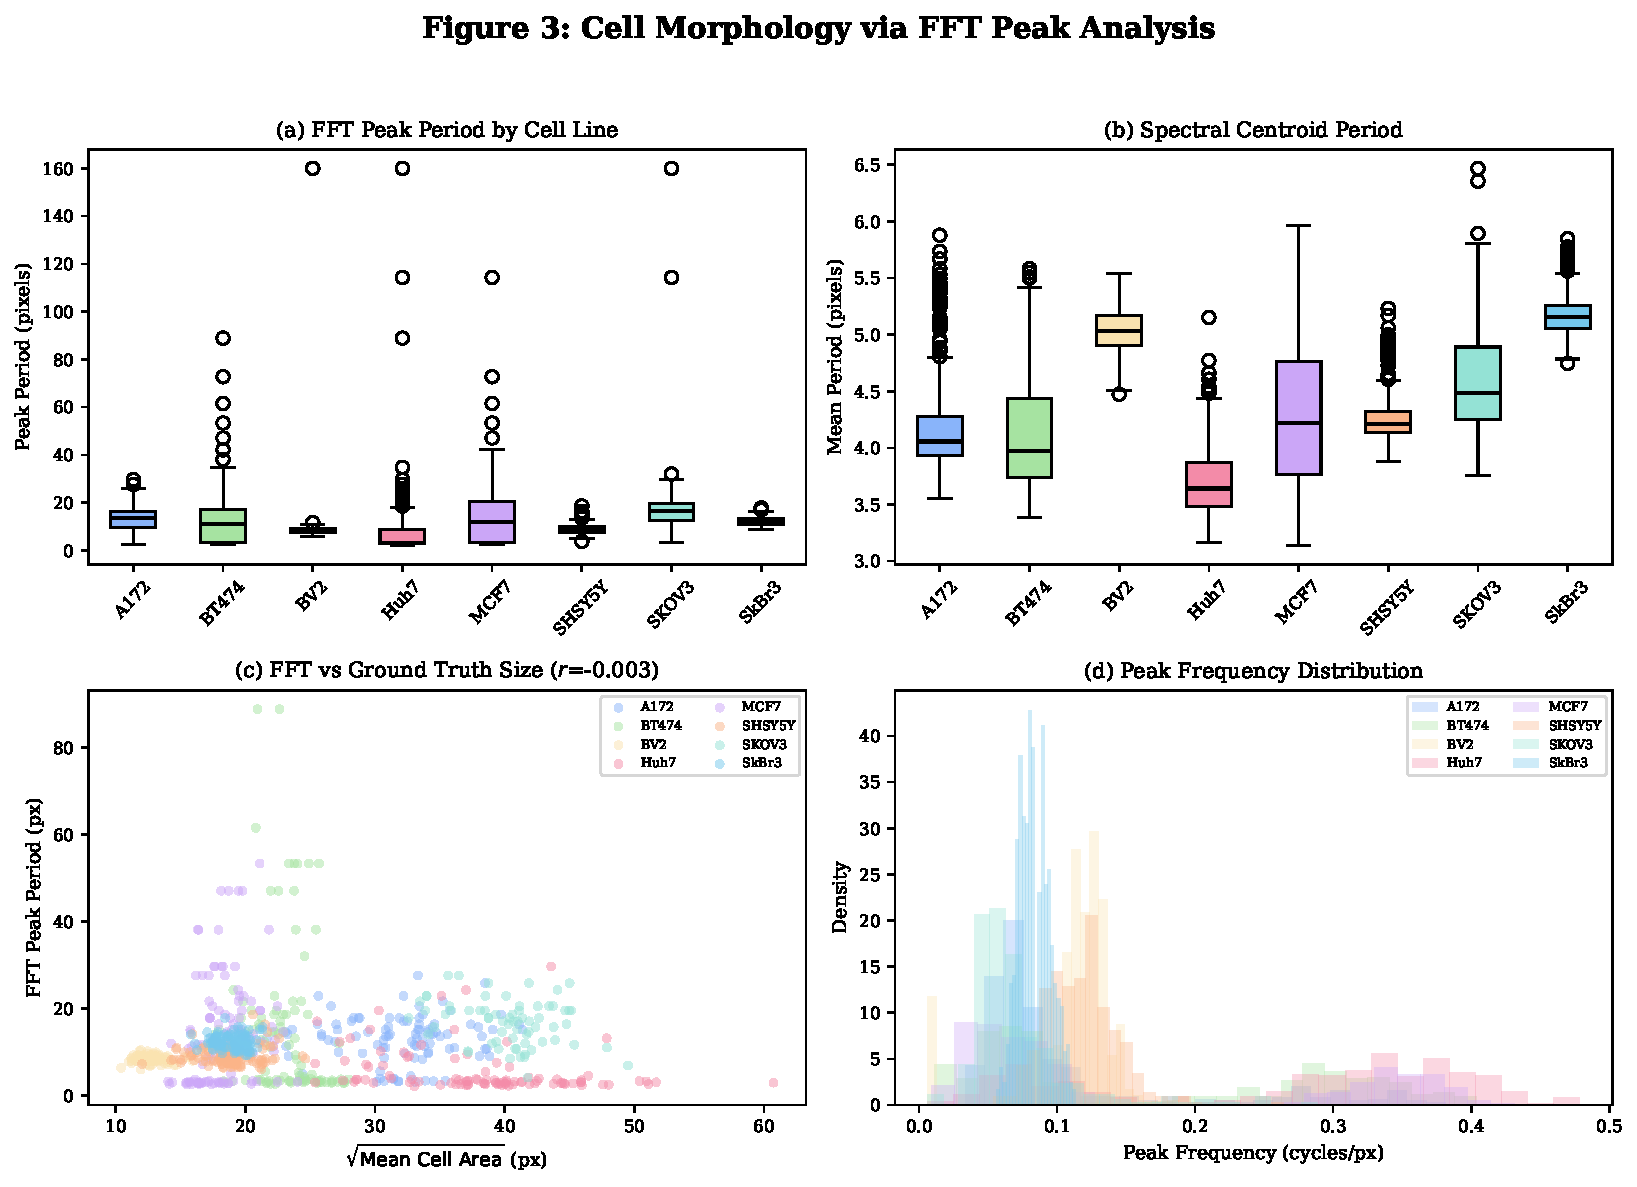
\includegraphics[width=\textwidth]{outputs/report_fig3_morphology.pdf}
    \caption{\textbf{Cell morphology via FFT peak analysis.} (a) FFT peak period
    distribution per cell line. (b) Spectral centroid period per cell line.
    (c) FFT peak period vs.\ ground truth $\sqrt{\text{cell area}}$ from COCO
    annotations. (d) Peak frequency distributions.}
    \label{fig:morphology}
\end{figure}

The correlation between FFT peak period and ground truth cell area was weak
($r = -0.016$, Fig.~\ref{fig:morphology}c), indicating that simple FFT peak
analysis is insufficient for accurate cell size estimation in phase-contrast
images. This is expected due to the complex contrast transfer function of
phase-contrast optics, which produces halo artifacts that dominate the
high-frequency content.

\subsection{Image Quality \& Artifact Detection}

All images exhibited high isotropy (isotropy $\approx 1.0$), indicating minimal
directional artifacts. The low-frequency power fraction, a proxy for background
shading, ranged from 1.6\% (SHSY5Y) to 6.6\% (BV2), indicating generally good
illumination uniformity across the dataset.

\subsection{Cell Line Classification}

Using 94 FFT features per image, we achieved 81.7\% classification accuracy
across 8 cell lines with a support vector machine (SVM) using an RBF kernel
(5-fold stratified cross-validation). Random Forest achieved 81.4\% and
Logistic Regression 80.4\% (Fig.~\ref{fig:classification}a).

\begin{figure}[H]
    \centering
    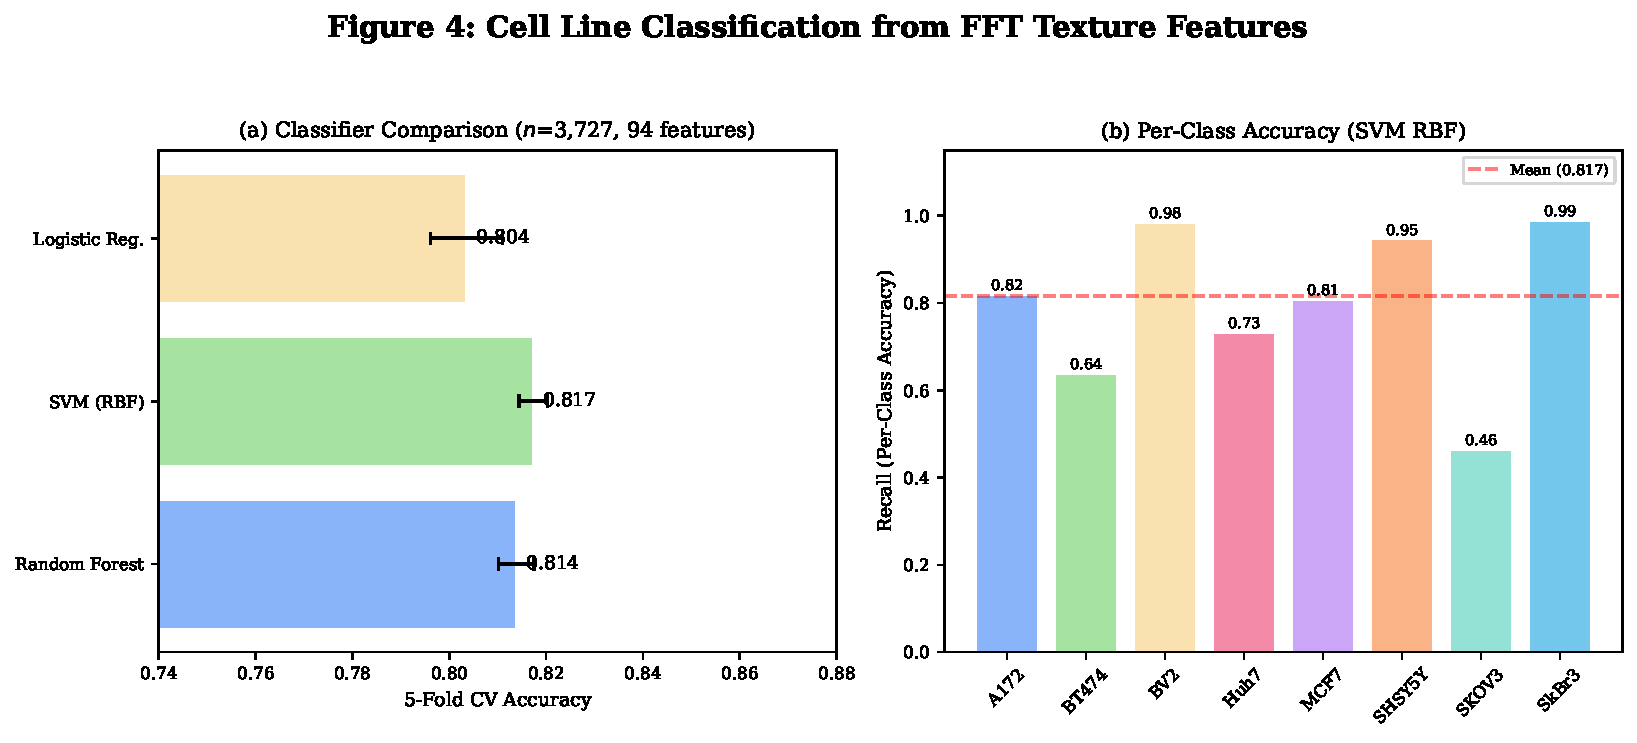
\includegraphics[width=\textwidth]{outputs/report_fig4_classification.pdf}
    \caption{\textbf{Cell line classification from FFT texture features.}
    (a) Classifier comparison (5-fold CV accuracy). (b) Per-class recall for
    SVM (RBF kernel). Feature vector: 94 dimensions (50 radial + 36 azimuthal
    + 8 scalar features).}
    \label{fig:classification}
\end{figure}

Per-class analysis (Fig.~\ref{fig:classification}b) revealed that BV2 (98.5\%),
SkBr3 (98.9\%), and SHSY5Y (94.7\%) were classified with high accuracy, while
SKOV3 (46.4\%) and BT474 (63.9\%) showed lower performance. SKOV3, the smallest
cell line, was frequently confused with debris and imaging artifacts. BT474 shares
morphological similarities with other breast cancer lines (MCF7, SkBr3).

\subsection{FFT-Based Segmentation Preprocessing}

Frequency-domain bandpass filtering improved Otsu thresholding segmentation
IoU from 0.325 (raw) to 0.394 (filtered), a mean improvement of $+0.070$
(Fig.~\ref{fig:segmentation}a). Of 808 annotated images, 332 (41.1\%) showed
improvement.

\begin{figure}[H]
    \centering
    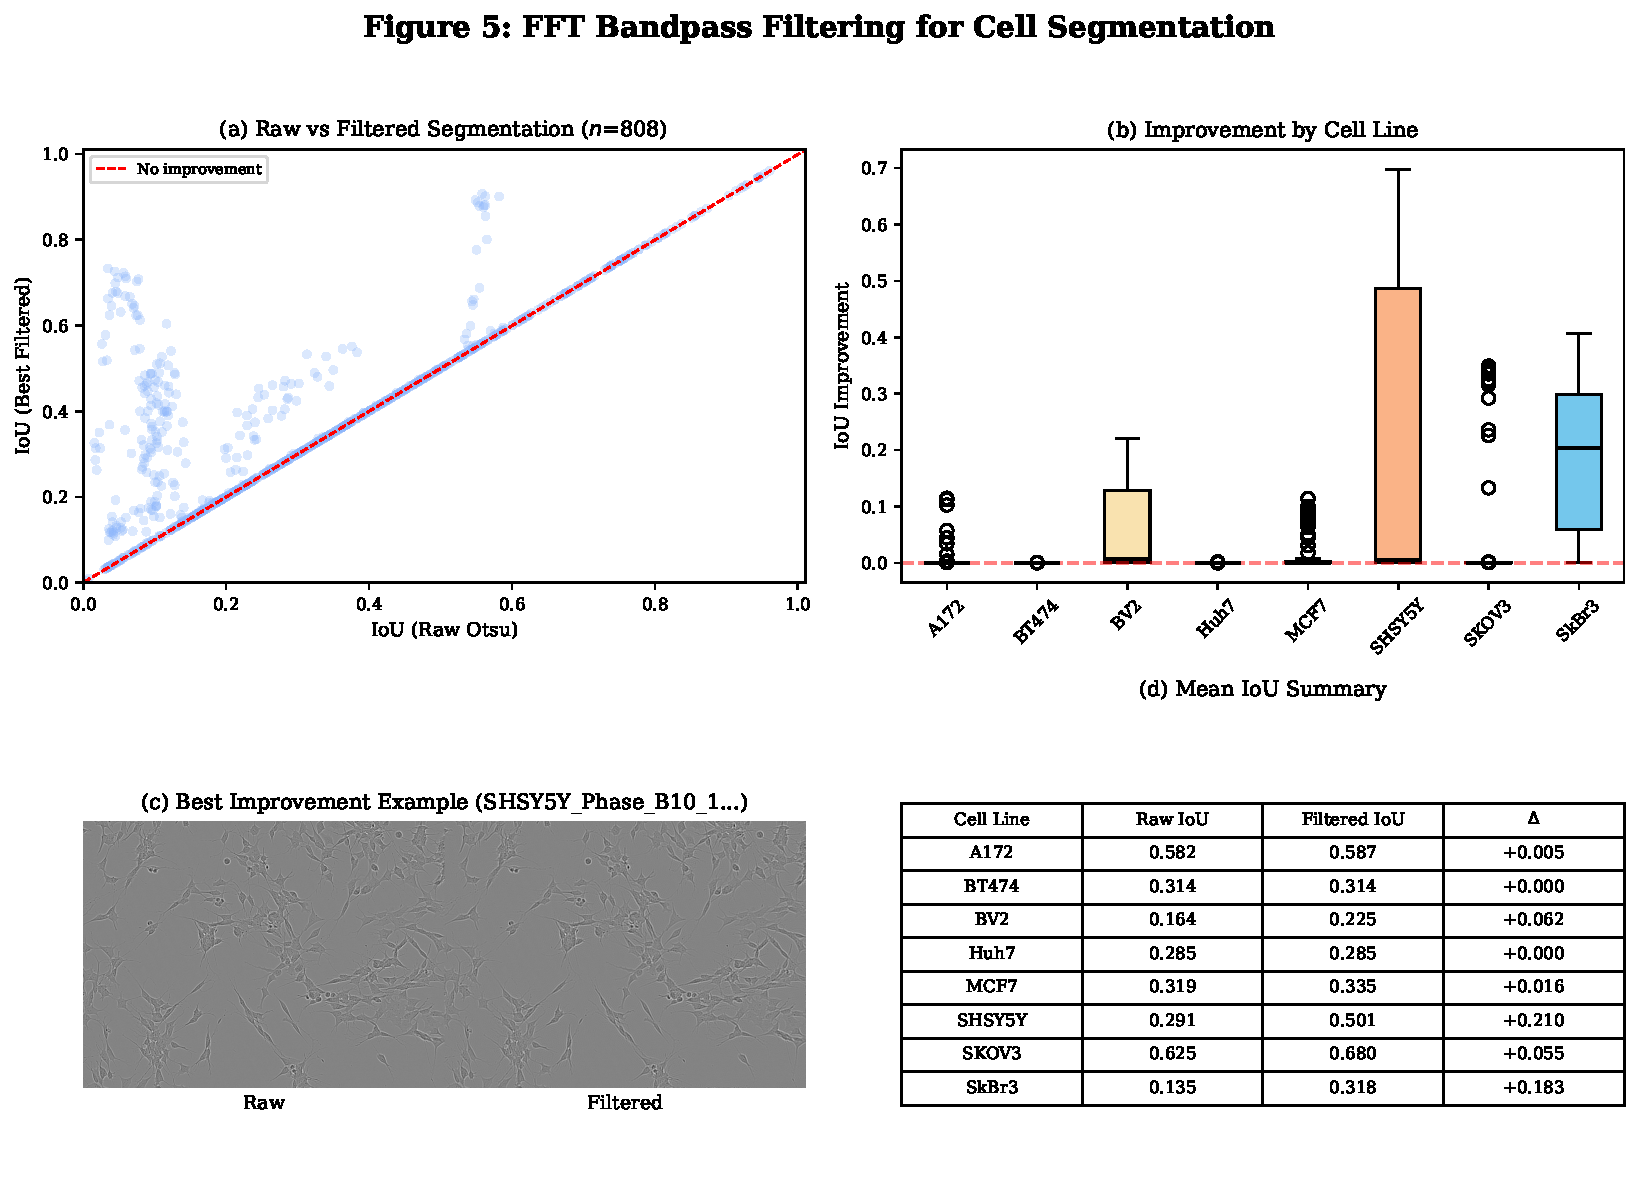
\includegraphics[width=\textwidth]{outputs/report_fig5_segmentation.pdf}
    \caption{\textbf{FFT bandpass filtering for segmentation.} (a) Raw vs.\
    filtered IoU scatter plot. (b) IoU improvement distribution per cell line.
    (c) Example of raw (left) and filtered (right) image with best improvement.
    (d) Mean IoU summary table.}
    \label{fig:segmentation}
\end{figure}

The improvement varied by cell line (Fig.~\ref{fig:segmentation}b,d): SHSY5Y
showed the largest gain ($\Delta\text{IoU} = +0.210$) while BT474 and Huh7
showed negligible improvement. This likely reflects the relative strength of
background unevenness in different cell lines.

\subsection{Time-Lapse Dynamics}

Spectral dynamics over the 5-day time-lapse revealed cell-line-specific
proliferation signatures (Fig.~\ref{fig:timelapse}). Total FFT power increased
over time for all lines (Fig.~\ref{fig:timelapse}b), consistent with increasing
cell confluence. The spectral centroid showed divergent trends: MCF7 and Huh7
exhibited increasing centroid (cells becoming smaller/more packed), while BV2
and SKOV3 showed decreasing centroid (cells spreading).

\begin{figure}[H]
    \centering
    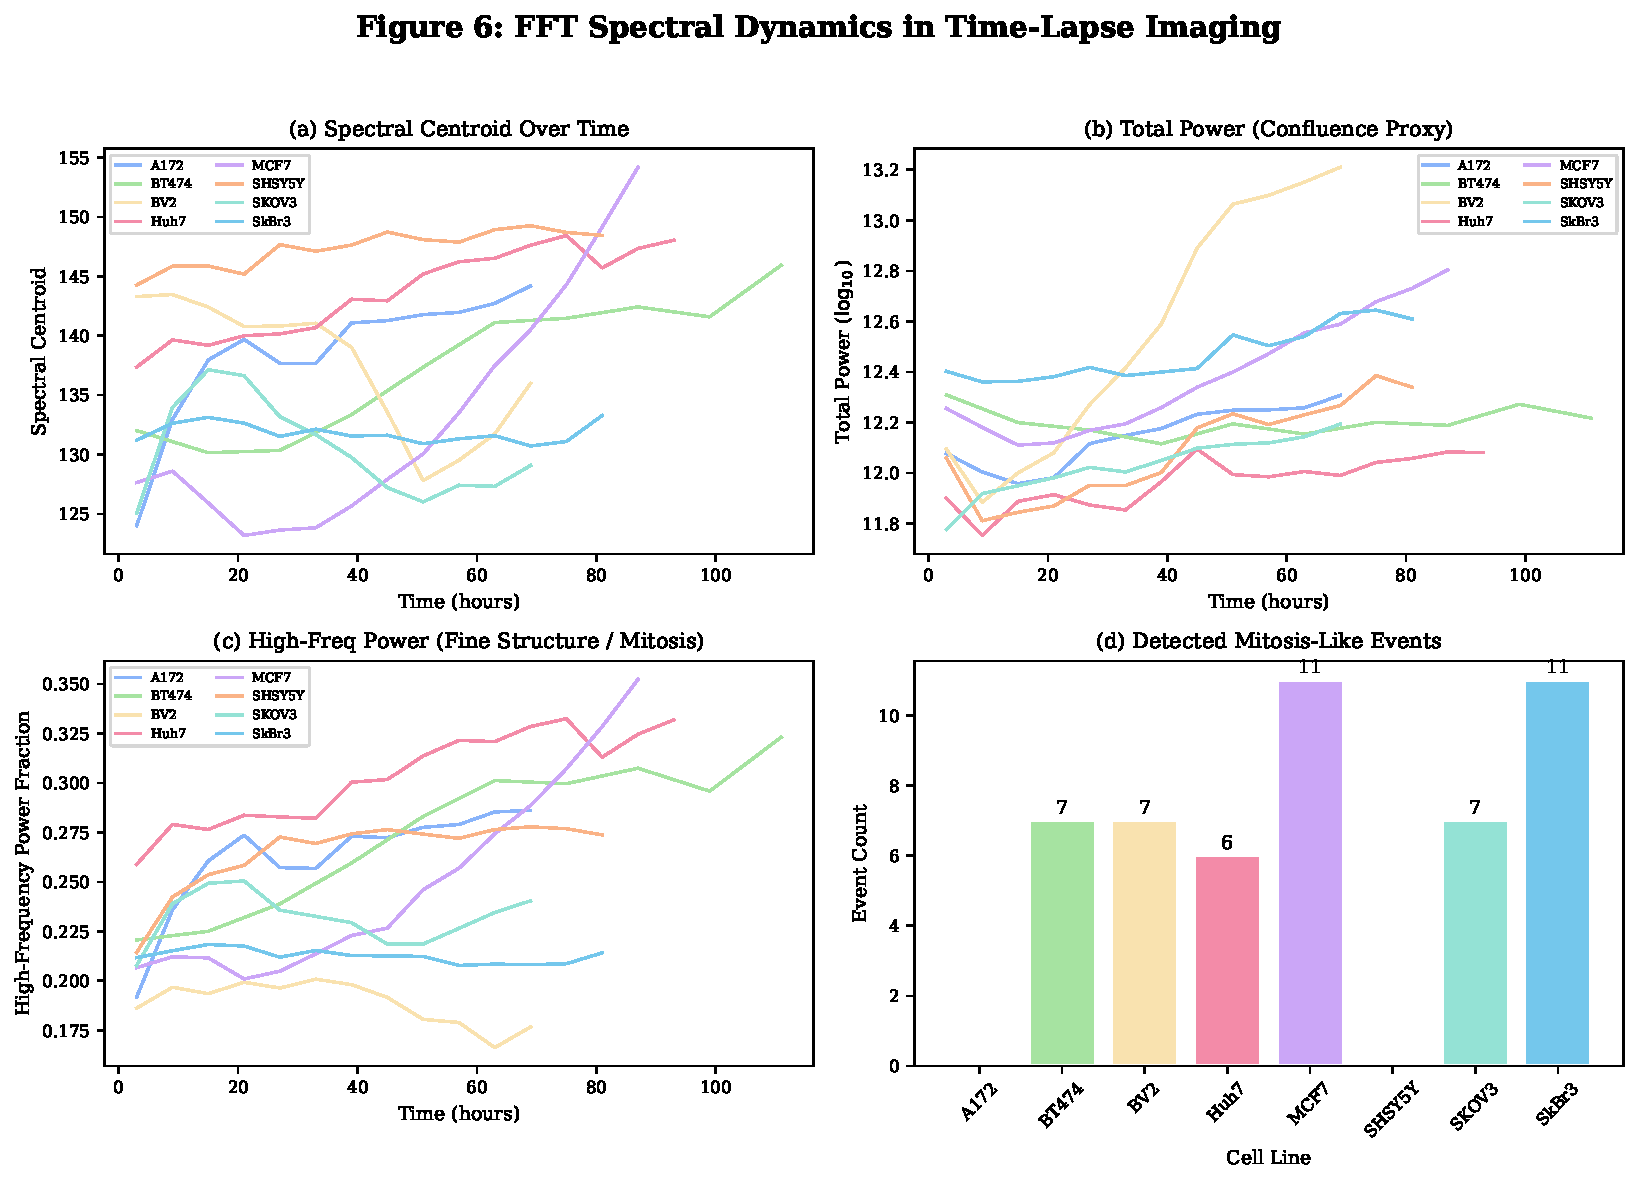
\includegraphics[width=\textwidth]{outputs/report_fig6_timelapse.pdf}
    \caption{\textbf{FFT spectral dynamics in time-lapse imaging.} (a) Spectral
    centroid over time (6-hour bins). (b) Total power over time (confluence proxy).
    (c) High-frequency power over time (fine structure/mitosis proxy).
    (d) Detected mitosis-like events per cell line.}
    \label{fig:timelapse}
\end{figure}

Mitosis-like events, detected as spikes in high-frequency power, totaled 49
across all wells (Fig.~\ref{fig:timelapse}d). MCF7 and SkBr3 showed the most
events (11 each), consistent with their rapid proliferation rates. A172 and
SHSY5Y showed zero events, consistent with their slower growth kinetics.

\section{Discussion}

Our results demonstrate that FFT analysis provides a rich, label-free
characterization of phase-contrast microscopy images. The strong correlation
between total FFT power and cell density ($r = 0.751$) suggests that integrated
power spectral density can serve as a rapid, annotation-free proxy for cell
confluence---a metric of practical importance in high-throughput screening.

The 81.7\% classification accuracy from FFT features alone is notable given
that no spatial or morphological features were used. The misclassification
patterns (SKOV3 confused with artifacts, BT474 confused with other breast
cancer lines) are consistent with known morphological similarities and suggest
that combining FFT features with spatial features could improve performance.

The modest but consistent segmentation improvement from bandpass filtering
($\Delta\text{IoU} = +0.070$) demonstrates that frequency-domain preprocessing
can enhance downstream analysis pipelines. The cell-line-dependent improvement
suggests that filter parameters should be optimized per cell line for best
results.

Time-lapse FFT dynamics reveal biological insights: the increasing total power
tracks confluence, while spectral centroid shifts reflect changes in cell
morphology during growth. The mitosis detection approach, while simple,
successfully identified proliferating vs.\ quiescent cell lines.

\subsection{Limitations}

Several limitations should be noted. First, the FFT peak period showed poor
correlation with ground truth cell area, likely due to the complex contrast
transfer function of phase-contrast optics. Second, the isotropy analysis
showed uniformly high values, limiting its utility as a quality discriminator.
Third, the mitosis detection method is heuristic and may miss events or produce
false positives. Fourth, the 25\% annotation subset limits the statistical power
of cell-count-based analyses.

\subsection{Future Work}

Future directions include: (1) combining FFT features with deep learning
embeddings for improved classification, (2) developing cell-line-adaptive
filter designs, (3) extending the time-lapse analysis to track individual
wells rather than population averages, and (4) applying the framework to
other microscopy modalities (fluorescence, DIC).

\section{Conclusion}

We presented a comprehensive FFT analysis of 3,727 phase-contrast microscopy
images across 8 cell lines. Key findings include: total FFT power as a
strong cell density proxy ($r = 0.751$), 81.7\% cell line classification
accuracy from FFT texture features, segmentation improvement through
bandpass filtering ($\Delta\text{IoU} = +0.070$), and cell-line-specific
time-lapse proliferation signatures. These results establish FFT analysis
as a valuable, computationally efficient tool for quantitative phase-contrast
microscopy.

\section*{Data Availability}

Analysis code and results are available at
\url{https://github.com/mjonyh/microscopic_images}.

\section*{Acknowledgments}

This work was performed using the LIVECell dataset
(Edlund et al., 2021, Nature Methods) via Kaggle.

\begin{thebibliography}{9}
\bibitem{castleman1979} Castleman, K.R. (1979). \textit{Digital Image
    Processing}. Prentice-Hall.
\bibitem{lloyd1993} Lloyd, D. et al. (1993). The cell nucleus in
    perspective. \textit{Trends in Cell Biology}, 3(11), 390--392.
\bibitem{bray2012} Bray, M.-A. et al. (2012). Cell Painting, a
    high-content image-based assay for morphological profiling.
    \textit{Nature Protocols}, 7, 1747--1761.
\bibitem{edlund2021livecell} Edlund, C. et al. (2021). LIVECell---A
    large-scale dataset for label-free live cell segmentation.
    \textit{Nature Methods}, 18, 1048--1057.
\end{thebibliography}

\end{document}
